%%%%%%%%%%%%%%%%%%%% author2.tex %%%%%%%%%%%%%%%%%%%%%%%%%%%%%%%%%%%
%
% IEEE-style paper restructured to standard research headings
%
%%%%%%%%%%%%%%%% IEEE %%%%%%%%%%%%%%%%%%%%%%%%%%%%%%%%%%

\documentclass[conference]{IEEEtran}

% Force numeric author reference marks (1,2,3,...) instead of symbol marks (*,†,‡,...)
\makeatletter
\renewcommand{\IEEEauthorrefmark}[1]{\textsuperscript{#1}}
\makeatother

% to typeset URLs, URIs, and DOIs
\usepackage{url}
\usepackage{color}
\usepackage{graphicx}
\usepackage{tabularx}
\usepackage{multirow}
\usepackage{cite}
\usepackage{algorithm}
\usepackage{algorithmic}
\usepackage{longtable}
\usepackage{rotating}
\usepackage{placeins}
\usepackage{amsmath}
\usepackage{amssymb}
\def\UrlFont{\rmfamily}

\begin{document}

\title{ML-Based Decision Support System\\for Smart Investments}
\author{\IEEEauthorblockN{Dr. Reshma Koli\IEEEauthorrefmark{1}, Avanish Vadke\IEEEauthorrefmark{2}, Atharva Shelke\IEEEauthorrefmark{3},\\Abhishek Thormothe\IEEEauthorrefmark{4}, Aadit Suryawanshi\IEEEauthorrefmark{5},\\Prof. Harshada Sonkamble\IEEEauthorrefmark{6}}
\IEEEauthorblockA{\IEEEauthorrefmark{1}\IEEEauthorrefmark{2}\IEEEauthorrefmark{3}\IEEEauthorrefmark{4}\IEEEauthorrefmark{5}\IEEEauthorrefmark{6}A.P. Shah Institute of Technology, Thane, India\\
rrkoli@apsit.edu.in, avanishvadke3@apsit.edu.in,\\
atharvashelke2@apsit.edu.in, abhishekthormothe150@apsit.edu.in,\\
aaditsuryavanshi60@apsit.edu.in, hksonkamble@apsit.edu.in}}

\maketitle

\begin{abstract}
Retail investors and discretionary traders make investment decisions under uncertainty, limited information, and behavioral bias. This work presents \emph{QuantFin}, a machine learning--based decision support system for equity investments over Indian large-cap stocks (Nifty~50 constituents available in the repository dataset). The system operationalizes a reproducible workflow: ingestion of daily OHLCV time series from multi-header CSV exports; technical-indicator feature engineering; training and inference across multiple model families (ridge regression, logistic regression, support vector machines (SVM), ARIMA, and long short-term memory (LSTM)); ML-driven ranking for portfolio selection; periodic rebalancing; and leakage-aware walk-forward backtesting against an equal-weight benchmark.

Quantitative results are reported strictly from repository artifacts and the implemented backtest engine. For example, on the RELIANCE dataset, saved training metrics show test accuracy of 0.5003 (logistic regression) and 0.5136 (SVM) for directional classification, and LSTM test MAPE of 20.447\% for price forecasting. In a reproducible walk-forward run (monthly rebalancing, 2023-01-01 to 2024-01-01), the implemented LINEAR strategy achieved CAGR 48.31\% versus 30.60\% for the benchmark under the repository's backtest assumptions.
\end{abstract}

\begin{IEEEkeywords}
Decision Support Systems, Quantitative Finance, Portfolio Construction, Walk-Forward Backtesting, Time Series Forecasting, Nifty~50
\end{IEEEkeywords}

\section{Introduction}\label{sec:intro}
Quantitative investing systems increasingly combine statistical modeling, machine learning, and portfolio construction, but reported performance is sensitive to evaluation protocol: time-order must be respected and realistic constraints (e.g., rebalancing cadence and budget) must be explicit. QuantFin is designed as a full-stack platform that connects these components for the Indian equity universe (Nifty~50 constituents available in the repository dataset). Unlike isolated notebooks, QuantFin operationalizes a repeatable workflow: (i) ingestion of OHLCV data from CSV exports with robust header handling; (ii) technical indicator generation; (iii) model training and prediction orchestration across multiple approaches; (iv) portfolio construction and rebalancing; and (v) walk-forward backtesting with a benchmark.

\textbf{Problem statement.} Retail-facing investment tooling often lacks (a) a transparent, end-to-end data-to-decision pipeline and (b) leakage-aware evaluation that ties predictions to realized returns under a rebalance schedule. This creates a gap between model metrics (accuracy/MAE) and investment outcomes (drawdown, Sharpe).

\textbf{Objectives.} QuantFin aims to provide an end-to-end decision support workflow with clear interfaces (APIs), multiple model baselines, and walk-forward evaluation.

\textbf{Contributions.} This work contributes:
\begin{itemize}
\item An end-to-end, modular architecture (FastAPI backend + React/Vite dashboard) for interactive quantitative analysis.
\item A leakage-aware walk-forward backtesting procedure that enforces date cutoffs at each rebalance date and reports risk-adjusted metrics.
\item A multi-model prediction layer and portfolio construction baselines implemented in the repository.
\end{itemize}

\textbf{Organization.} Section~\ref{sec:rw} reviews related work; Section~\ref{sec:form} formalizes the system model; Section~\ref{sec:method} describes the proposed methodology; Section~\ref{sec:arch} presents architecture and algorithms; Section~\ref{sec:impl} covers implementation details; Section~\ref{sec:setup} defines the experimental setup; and Section~\ref{sec:results} reports results and discussion.

\section{Related Work}\label{sec:rw}
This section links each design motivation to specific post-2020 research, and clarifies which idea is being adopted or contrasted.

\textbf{End-to-end ML portfolio decision support.} Aithal \emph{et al.}~\cite{aithal2023realtime} describe an IEEE Access real-time portfolio management system that integrates ML prediction with portfolio decisions. QuantFin adopts this end-to-end framing (data $\rightarrow$ model $\rightarrow$ decision $\rightarrow$ evaluation) but implements it as a lightweight FastAPI service with explicit walk-forward evaluation.

\textbf{Stock ranking and recommendation.} Saha \emph{et al.}~\cite{saha2021stockranking} study stock ranking prediction with list-wise approaches and embeddings. QuantFin similarly uses ranking as the decision interface (select top-$N$ candidates at each rebalance date), but uses a simpler score derived from predicted return and confidence to stay consistent with the repository's implementation.

\textbf{Classical vs deep time-series baselines.} Gao~\cite{gao2021arimadeep} benchmarks ARIMA against deep models for stock prediction. QuantFin follows this comparative-baseline idea by including ARIMA alongside LSTM, enabling users to compare a classical univariate model to a sequence model in the same pipeline.

\textbf{LSTM-based trend prediction.} Karlis \emph{et al.}~\cite{karlis2021lstmfusion} apply LSTM architectures for trend prediction by fusing multiple signals. QuantFin includes an LSTM pipeline with windowing and scaling; in the current repository state, the LSTM is used as a forecasting baseline rather than a fully fused multi-source model.

\textbf{Portfolio optimization baselines.} Gunjan and Bhattacharyya~\cite{gunjan2022portfolioreview} provide a Springer review of portfolio optimization methods. QuantFin includes mean--variance and risk-parity style baselines as reference points against the ML-driven ranking strategy, acknowledging that optimization quality depends on covariance estimation.

\textbf{Dynamic rebalancing and RL approaches.} Lim \emph{et al.}~\cite{lim2022dynamicrebalancing} and Ma \emph{et al.}~\cite{ma2023tcr} present reinforcement-learning based portfolio management and rebalancing. QuantFin does not implement RL, but uses their problem framing to motivate periodic rebalancing and evaluation under realistic sequences of decisions.

\textbf{Learning market structure.} Emekcio{\u{g}}lu and P{\i}nar~\cite{emekcioglu2023gnn} explore graph neural networks for portfolio optimization. QuantFin currently uses a simpler feature-based approach; the GNN line of work motivates future extensions when cross-asset structure is explicitly modeled.

\section{System Model / Problem Formulation}\label{sec:form}
Let $\mathcal{S}=\{1,\dots,N\}$ be the universe of tradable symbols (Nifty~50 constituents available in the dataset). Let $D = (d_0, d_1, \dots, d_T)$ be rebalance dates with $d_{t} < d_{t+1}$. At each rebalance date $d_t$, the system computes features from data up to $d_t$ and produces a per-asset predicted return $\widehat{r}_{i,t}$ and a confidence score $c_{i,t}\in[0,1]$.

\subsection{Ranking-based selection}
QuantFin's ML-driven ranking uses the score
\begin{equation}
\mathrm{score}_{i,t} = \widehat{r}_{i,t} \cdot c_{i,t}
\end{equation}
filters assets with $\widehat{r}_{i,t} \le 0$, selects the top-$K$ assets, and assigns equal weights among selected assets (as implemented in the backtest router):
\begin{equation}
 w_{i,t} =
 \begin{cases}
  1/K, & i \in \mathrm{TopK}(\mathrm{score}_{\cdot,t}) \\
  0, & \text{otherwise.}
 \end{cases}
\end{equation}
The portfolio value evolves by realized returns over each rebalance interval.

\subsection{Benchmark definition}
The benchmark is an equal-weighted portfolio of all available symbols, computed over the same rebalance periods. This makes the comparison aligned in both time and rebalancing cadence.

\subsection{Assumptions and constraints}
The repository backtest assumes (i) long-only allocation, (ii) discrete rebalancing at fixed cadence, and (iii) no explicit transaction costs or slippage. These constraints are stated to avoid over-claiming.

\section{Methodology / Proposed Method}\label{sec:method}
QuantFin's methodology is a modular pipeline:
\begin{enumerate}
\item \textbf{Data ingestion:} load per-symbol OHLCV CSV files and normalize headers to a canonical schema.
\item \textbf{Feature engineering:} compute return-based and indicator-based features (e.g., SMA/EMA, MACD, RSI, Bollinger bands, rolling volatility).
\item \textbf{Model training and inference:} train/serve multiple model families for regression and classification.
\item \textbf{Decision support:} convert predictions into rankings/allocations under a capital budget.
\item \textbf{Walk-forward evaluation:} simulate rebalancing over time using only information available at each rebalance date.
\end{enumerate}

Given close price $P_t$, simple returns and log-returns are:
\begin{equation}
 r_t = \frac{P_t - P_{t-1}}{P_{t-1}},\quad \ell_t = \log\left(\frac{P_t}{P_{t-1}}\right)
\end{equation}
These, along with indicators, form the model input matrix.

\subsection{Feature engineering details (repo-implemented indicators)}
QuantFin computes multiple technical indicators directly from OHLCV series. Below we summarize common indicator definitions aligned with the repository implementations.

\textbf{Moving averages.} For window $w$, the simple moving average (SMA) is
\begin{equation}
\mathrm{SMA}_w(t)=\frac{1}{w}\sum_{k=0}^{w-1} P_{t-k}.
\end{equation}
The exponential moving average (EMA) uses smoothing factor $\alpha=\tfrac{2}{w+1}$:
\begin{equation}
\mathrm{EMA}_w(t)=\alpha P_t + (1-\alpha)\mathrm{EMA}_w(t-1).
\end{equation}

\textbf{RSI.} Let $\Delta_t=P_t-P_{t-1}$ and define average gains/losses over a window $w$ as $G_w$ and $L_w$ (with $G_w\ge 0$, $L_w\ge 0$). The relative strength is $\mathrm{RS}=\tfrac{G_w}{L_w}$ and
\begin{equation}
\mathrm{RSI}=100-\frac{100}{1+\mathrm{RS}}.
\end{equation}

\textbf{MACD.} With fast and slow EMAs, $\mathrm{EMA}_{12}$ and $\mathrm{EMA}_{26}$,
\begin{equation}
\mathrm{MACD}=\mathrm{EMA}_{12}-\mathrm{EMA}_{26},\quad \mathrm{Signal}=\mathrm{EMA}_9(\mathrm{MACD}).
\end{equation}

\textbf{Bollinger bands.} With $m=\mathrm{SMA}_{20}$ and rolling standard deviation $\sigma_{20}$,
\begin{equation}
\mathrm{Upper}=m+2\sigma_{20},\quad \mathrm{Lower}=m-2\sigma_{20}.
\end{equation}

\begin{table*}[!t]
\centering
\caption{Representative engineered indicators used by QuantFin (implemented in repository services).}
\label{tab:features}
\small
\renewcommand{\arraystretch}{1.15}
\setlength{\tabcolsep}{6pt}
\begin{tabularx}{\textwidth}{|l|l|X|}
\hline
\textbf{Feature family} & \textbf{Examples (typical params)} & \textbf{Purpose / intuition}\\
\hline
Returns & $r_t$, $\ell_t$, lagged returns & Captures short-horizon momentum/mean-reversion signals and stabilizes modeling via log-returns.\\
Trend & SMA/EMA (multiple windows), momentum features & Encodes direction and trend persistence at different time scales.\\
Oscillators & RSI (windowed gains/losses) & Measures overbought/oversold regimes from relative gain vs loss.\\
Mean reversion bands & Bollinger bands (20-day mean and variance) & Captures deviation from rolling mean scaled by volatility.\\
Cross-over signals & MACD and MACD signal & Encodes trend change via fast/slow EMA cross-overs.\\
Volume & Volume SMA, volume ratio & Provides liquidity/activity proxy and filters price-only signals.\\
\hline
\end{tabularx}
\end{table*}

\section{Algorithm / Architecture Design}\label{sec:arch}
\subsection{System architecture}
QuantFin is implemented as a modular full-stack system:
\begin{itemize}
\item \textbf{Backend:} a FastAPI service exposing endpoints for portfolio rebalancing, analytics (training + metrics), predictions, and walk-forward backtesting.
\item \textbf{Model services:} reusable components for preprocessing, features, training, inference, and allocation.
\item \textbf{Frontend:} a React + TypeScript dashboard (Vite) consuming backend APIs.
\end{itemize}

\begin{figure}[!t]
\begin{center}
\fbox{\parbox{0.95\columnwidth}{
\textbf{QuantFin Architecture (conceptual).}\\
\emph{Data layer:} CSV OHLCV $\rightarrow$ preprocessing $\rightarrow$ feature engineering.\\
\emph{Model layer:} Linear, Logistic, SVM, ARIMA, and LSTM models with an ensemble option.\\
\emph{Decision layer:} ranking/weighting $\rightarrow$ rebalancing $\rightarrow$ backtesting.\\
\emph{Serving layer:} FastAPI endpoints consumed by a React dashboard.
}}
\caption{QuantFin system architecture.}
\label{fig:arch}
\end{center}
\end{figure}

\subsection{Leakage-aware rebalancing algorithm}
\begin{algorithm}
\caption{Leakage-aware monthly rebalancing (simplified)}
\label{alg:rebalance}
\begin{algorithmic}
\STATE Input: universe $\mathcal{S}$, rebalance dates $D$, horizon $h$, top-$K$.
\STATE Initialize capital $V_0$.
\FOR{$t = 0$ to $|D|-2$}
\STATE Cutoff date $d \leftarrow D[t]$.
\STATE For each $i \in \mathcal{S}$: compute features using data $\le d$ and predict $\widehat{r}_{i,t}$.
\STATE Compute confidence $c_{i,t}$ from data quality/volatility/trend fit.
\STATE Rank by $\widehat{r}_{i,t} \cdot c_{i,t}$ and select top-$K$ with $\widehat{r}_{i,t} > 0$.
\STATE Allocate equal weights across selected assets; realize return over $(D[t], D[t+1]]$.
\ENDFOR
\STATE Output: portfolio value series and returns.
\end{algorithmic}
\end{algorithm}

\section{Implementation Details}\label{sec:impl}
\subsection{Dataset and storage}
QuantFin operates on daily OHLCV time series for Nifty~50 constituents stored as CSV files (one file per symbol) under the backend data directory. In the current repository state, the backend data directory contains 49 stock CSV files (excluding auxiliary files such as \texttt{nifty50.csv} and \texttt{tcs\_combined\_news.csv}). The global date range across these symbol files spans 1991-01-02 to 2025-10-06.

While an auxiliary news CSV exists at the repository root, it is excluded from the backend's stock-data loader and is not used by the current prediction or allocation flow.

\begin{table}[!t]
\centering
\caption{Repository dataset summary (computed from the backend data directory).}
\label{tab:dataset}
\small
\setlength{\tabcolsep}{4pt}
\renewcommand{\arraystretch}{1.15}
\begin{tabularx}{\columnwidth}{|X|c|}
\hline
\textbf{Property} & \textbf{Value}\\
\hline
Number of symbol CSV files & 49\\
Global date range & 1991-01-02 to 2025-10-06\\
Schema after normalization & Date, Open, High, Low, Close, Volume\\
Frequency & Daily bars (market days)\\
\hline
\end{tabularx}
\end{table}

\subsection{Software stack}
The backend is written in Python and served via FastAPI. The implementation uses common scientific Python libraries (NumPy, Pandas, scikit-learn, statsmodels, TensorFlow) and plotting utilities for analysis. The frontend is React + TypeScript built with Vite.

\subsection{API surface (backend)}
QuantFin exposes a REST API that maps closely to internal services. Table~\ref{tab:api} summarizes representative endpoint groups used by the dashboard and experiments.

\begin{table*}[!t]
\centering
\caption{Representative API endpoint groups in the QuantFin backend.}
\label{tab:api}
\small
\renewcommand{\arraystretch}{1.15}
\setlength{\tabcolsep}{6pt}
\begin{tabularx}{\textwidth}{|l|l|X|}
\hline
\textbf{Group} & \textbf{Prefix} & \textbf{Typical functionality}\\
\hline
Portfolio & \url{/api/portfolio} & Summary/performance series, portfolio health, rebalance workflows, cached strategy comparisons.\\
Analytics & \url{/api/analytics} & Training triggers and status, retrieval of cached metrics, candlestick/price-series endpoints backed by local OHLCV.\\
Predictions & \url{/api/predictions} & Per-symbol inference and portfolio recommendations parameterized by model family and prediction horizon.\\
Backtest & \url{/api/backtest} & Walk-forward evaluation via POST \url{/run}, returning portfolio/benchmark value series and risk metrics.\\
\hline
\end{tabularx}
\end{table*}

\subsection{Model suite}
QuantFin supports complementary model families:
\begin{itemize}
\item \textbf{Ridge regression:} $\ell_2$-regularized linear regression
\begin{equation}
\hat{\beta} = \arg\min_{\beta} \|y - X\beta\|_2^2 + \alpha\|\beta\|_2^2
\end{equation}
\item \textbf{Logistic regression:} directional classification
\begin{equation}
\Pr(y=1\mid x)=\sigma(w^\top x+b),\quad \sigma(z)=\frac{1}{1+e^{-z}}
\end{equation}
\item \textbf{SVM:} RBF-kernel classification baseline.
\item \textbf{ARIMA:} classical statistical baseline for univariate series.
\item \textbf{LSTM:} sequence model with gated updates
\begin{align}
 f_t &= \sigma(W_f[x_t,h_{t-1}] + b_f),\quad i_t = \sigma(W_i[x_t,h_{t-1}] + b_i),\\
 \tilde{c}_t &= \tanh(W_c[x_t,h_{t-1}] + b_c),\quad c_t = f_t\odot c_{t-1} + i_t\odot \tilde{c}_t,\\
 o_t &= \sigma(W_o[x_t,h_{t-1}] + b_o),\quad h_t = o_t\odot \tanh(c_t)
\end{align}
\end{itemize}

\section{Experimental Setup}\label{sec:setup}
\subsection{Evaluation protocol}
QuantFin evaluates strategies using walk-forward backtesting: at each rebalance date, predictions are generated using only historical data up to that date, a portfolio is formed, and realized returns are computed over the next period. This enforces a leakage-aware cutoff by construction.

\subsection{Backtest configuration (repo-grounded)}
The example backtest in this paper uses monthly rebalancing from 2023-01-01 to 2024-01-01, initial capital 100000, and top-$K=10$ selected assets under the LINEAR strategy. The benchmark is computed as an equal-weight basket across all available symbols over the same rebalance dates.

To increase external validity without changing the underlying implementation, we also report two additional configurations produced by the same backtest engine: (i) quarterly rebalancing over the same 2023-01-01 to 2024-01-01 window; and (ii) monthly rebalancing over a longer 2022-01-01 to 2024-01-01 window. These variants change only the evaluation horizon and/or rebalance cadence.

\subsection{Metrics}
Given a portfolio value series $V_t$ and periodic returns $r_t=\frac{V_t-V_{t-1}}{V_{t-1}}$, the implemented evaluation reports CAGR, Sharpe ratio, Sortino ratio, maximum drawdown, annualized volatility, Calmar ratio, and win rate.

\section{Results and Discussion}\label{sec:results}
\subsection{Sample model metrics}
Table~\ref{tab:metrics} reports sample metrics produced by QuantFin for the RELIANCE symbol (from an automated training run recorded in the repository). These metrics validate the end-to-end training and evaluation pipeline.

\begin{table*}[t]
\centering
\caption{Sample training metrics for a representative symbol (RELIANCE) from a recorded QuantFin run.}
\label{tab:metrics}
\small
\renewcommand{\arraystretch}{1.15}
\setlength{\tabcolsep}{6pt}
\begin{tabularx}{\textwidth}{|l|c|c|X|}
\hline
\textbf{Model} & \textbf{Test Acc.} & \textbf{Error (MAE/MAPE)} & \textbf{Notes} \\
\hline
Logistic Regression & 0.5003 & -- & Test AUC: 0.5073; test F1: 0.2779 \\
SVM (RBF) & 0.5136 & -- & Best params: $C=10.0,\gamma=0.01$; test AUC: 0.5051 \\
Ridge Regression & -- & MAE: 0.0742 & $\alpha=100.0$; test $R^2=-0.3354$ \\
LSTM & -- & MAPE: 20.447\% & Seq len: 60; units: [128,64]; dropout: 0.2 \\
\hline
\end{tabularx}
\end{table*}

\subsection{Walk-forward backtest example (strategy vs. benchmark)}
We ran the repository's walk-forward backtest engine with monthly rebalancing from 2023-01-01 to 2024-01-01 using the implemented LINEAR strategy (top 10, initial capital 100000). Under the repository's assumptions (no transaction costs or slippage), the strategy achieved CAGR 48.31\% versus 30.60\% for the benchmark, Sharpe 3.04 versus 1.75, and maximum drawdown -1.17\% versus -4.18\%. Final portfolio value was 148,271 versus 130,578 for the benchmark.

\begin{figure}[!t]
\centering
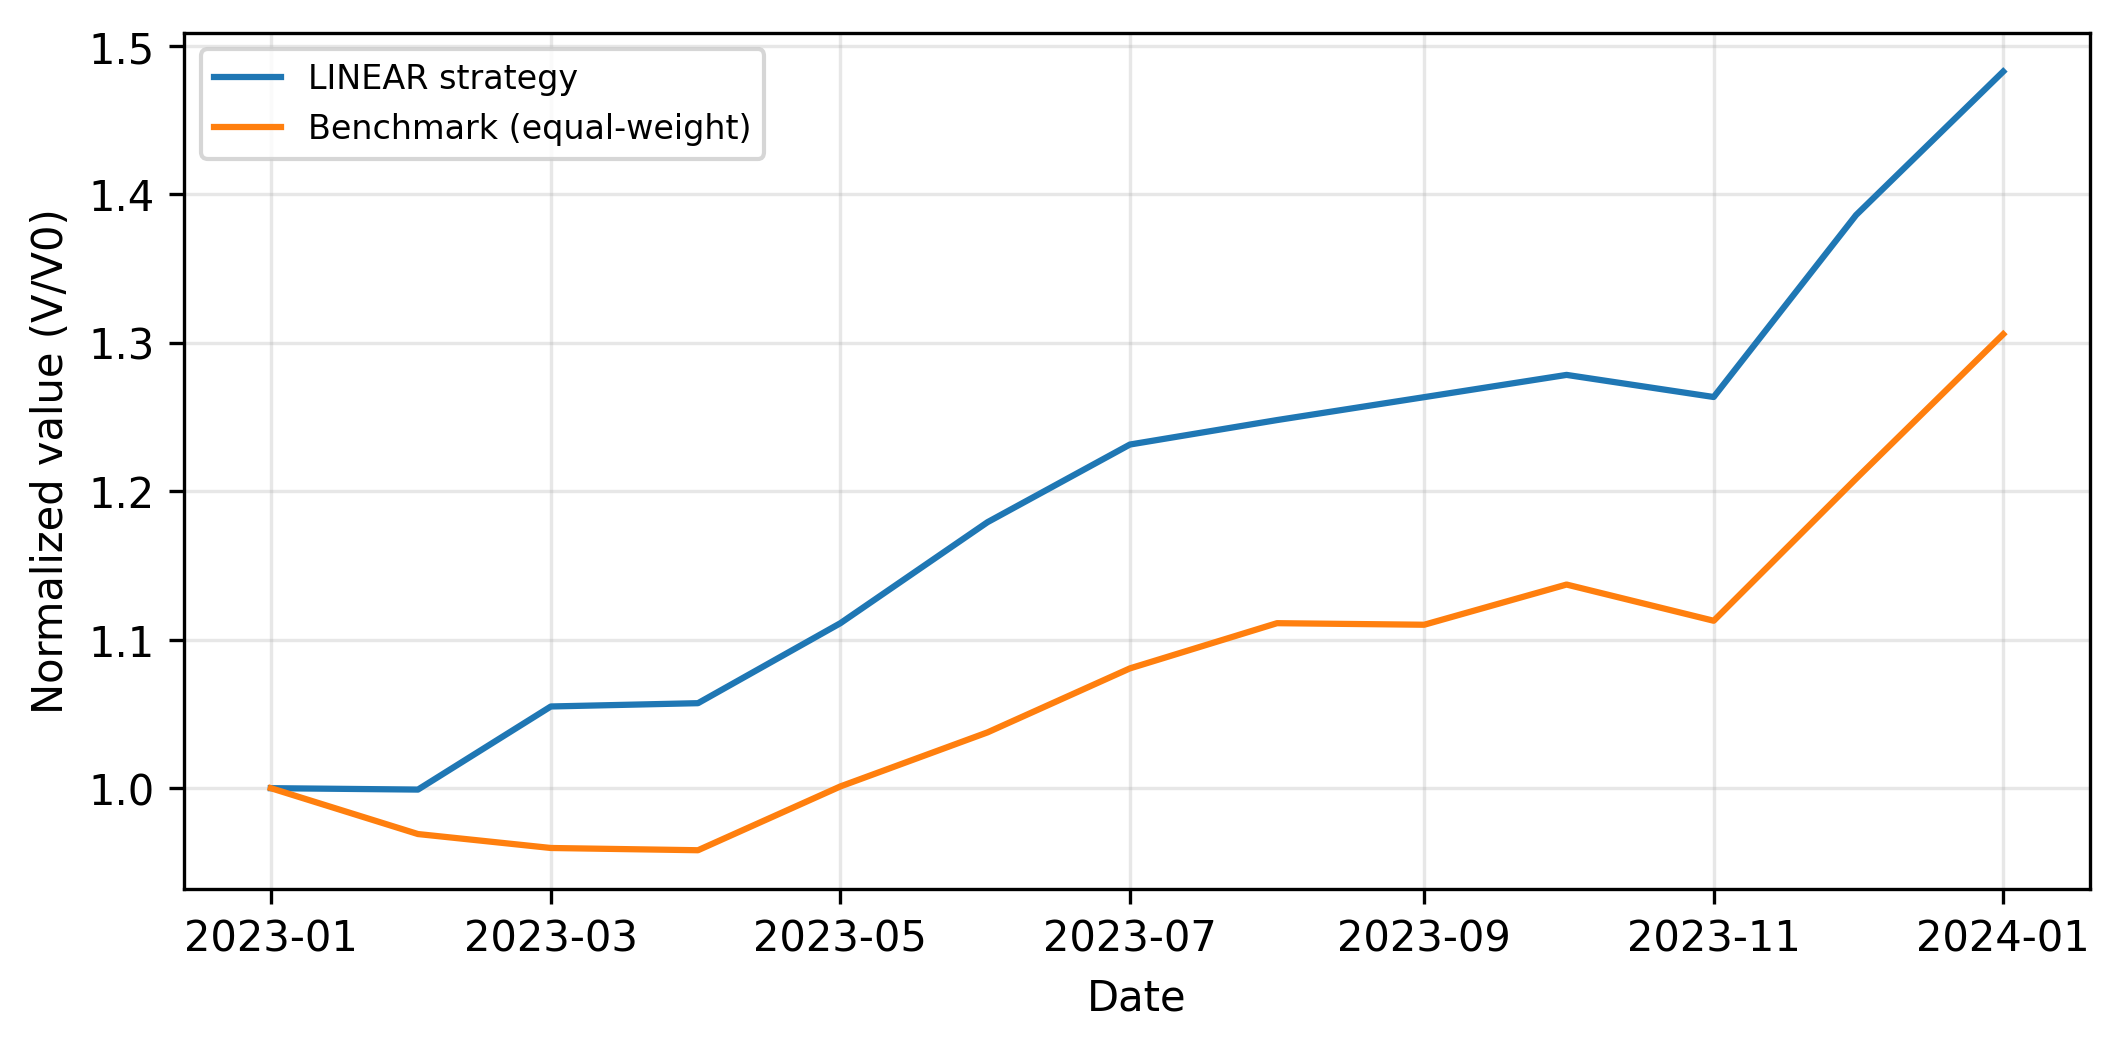
\includegraphics[width=\columnwidth]{figures/equity_curve_2023_2024_linear.png}
\caption{Normalized equity curve for the implemented LINEAR strategy vs. the equal-weight benchmark (monthly rebalancing, 2023-01-01 to 2024-01-01).}
\label{fig:equitycurve}
\end{figure}

\begin{figure}[!t]
\centering
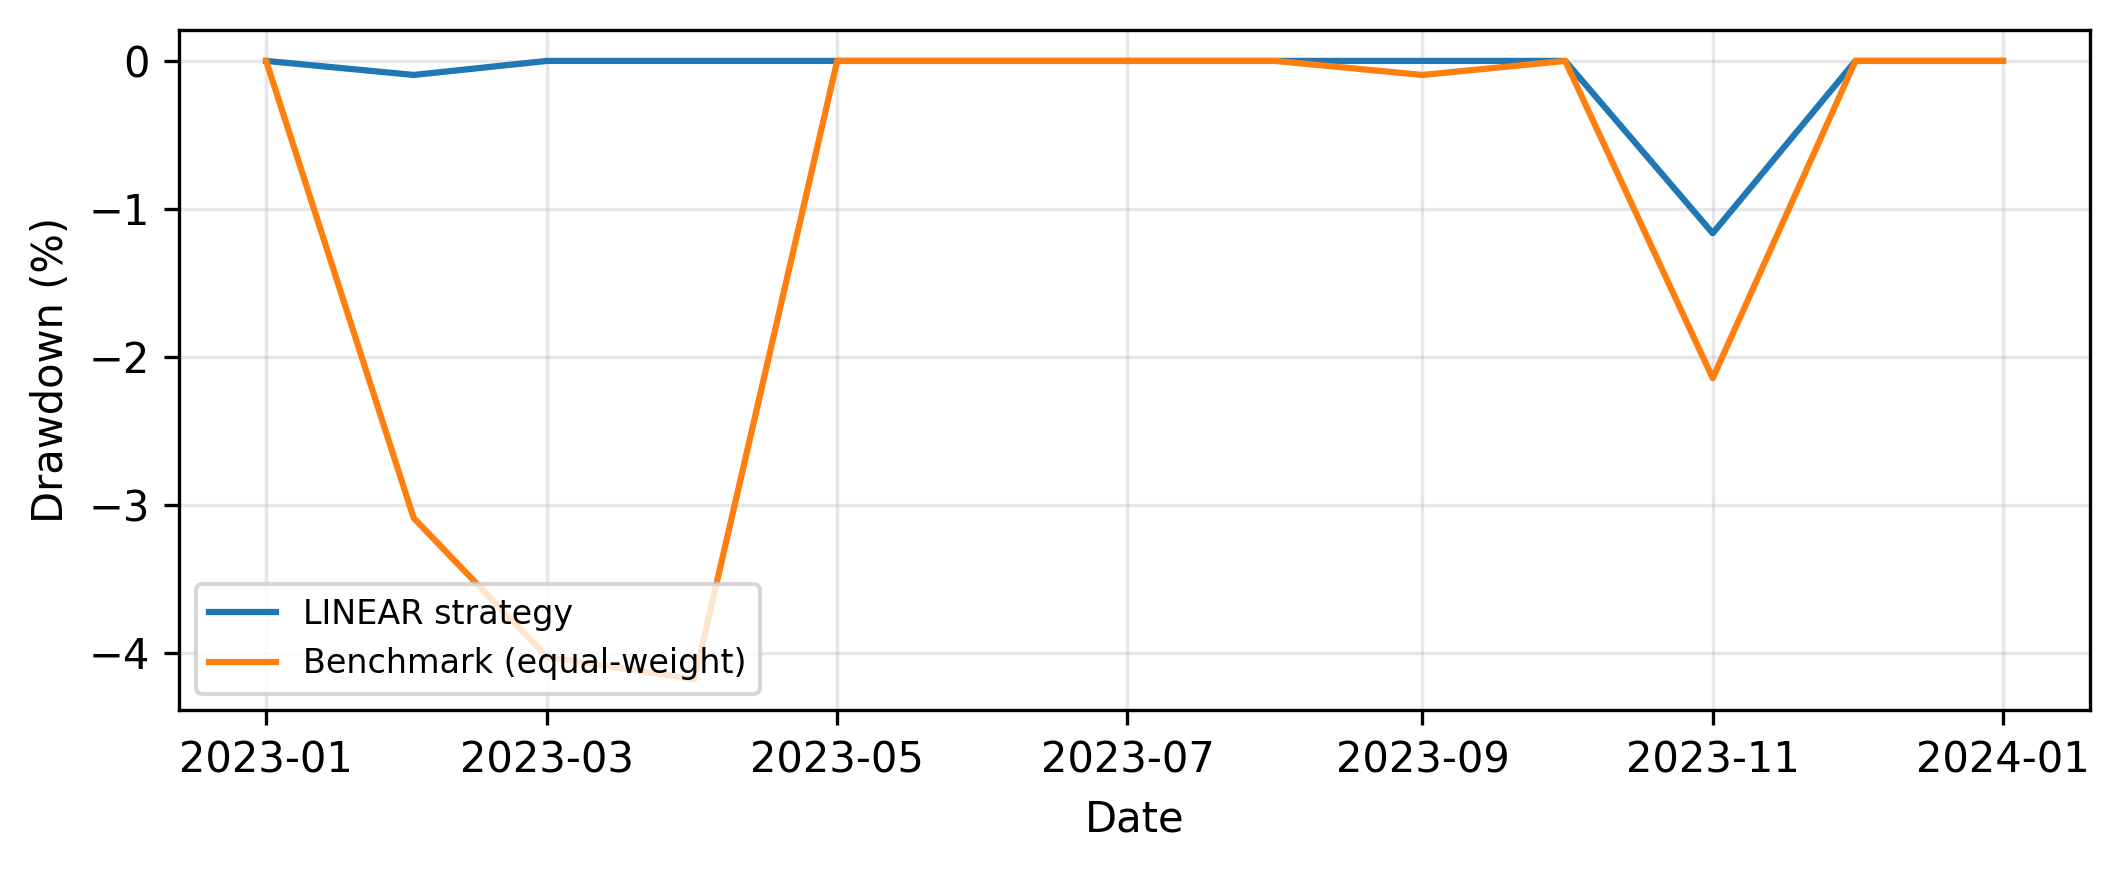
\includegraphics[width=\columnwidth]{figures/drawdown_2023_2024_linear.png}
\caption{Drawdown comparison for the implemented LINEAR strategy vs. the equal-weight benchmark over the same walk-forward run.}
\label{fig:drawdown}
\end{figure}

\begin{table}[!t]
\centering
\caption{Walk-forward backtest summary (monthly rebalancing, 2023-01-01 to 2024-01-01).}
\label{tab:backtest}
\small
\setlength{\tabcolsep}{4pt}
\renewcommand{\arraystretch}{1.15}
\begin{tabularx}{\columnwidth}{|X|c|c|c|}
\hline
\textbf{Portfolio} & \textbf{CAGR} & \textbf{Sharpe} & \textbf{Max DD} \\
\hline
LINEAR Strategy & 48.31\% & 3.04 & -1.17\% \\
Benchmark (equal-weight) & 30.60\% & 1.75 & -4.18\% \\
\hline
\end{tabularx}
\end{table}

\subsection{Additional backtest variants}
Table~\ref{tab:variants} reports additional repository-generated backtest variants. Quarterly rebalancing yields fewer evaluation periods (four quarters), so metrics that depend on downside samples (e.g., Sortino) can be unstable or undefined; therefore we emphasize CAGR, Sharpe, and maximum drawdown for cross-setting comparison.

\begin{table*}[!t]
\centering
\caption{Backtest variants produced by the repository engine (LINEAR strategy vs. equal-weight benchmark).}
\label{tab:variants}
\small
\renewcommand{\arraystretch}{1.15}
\setlength{\tabcolsep}{5pt}
\begin{tabularx}{\textwidth}{|X|c|c|c|c|}
\hline
\textbf{Variant} & \textbf{CAGR (S/B)} & \textbf{Sharpe (S/B)} & \textbf{Max DD (S/B)} & \textbf{Final value (S/B)}\\
\hline
Monthly (2023-01-01 to 2024-01-01) & 48.31/30.60 & 3.04/1.75 & -1.17/-4.18 & 148,272/130,578\\
Quarterly (2023-01-01 to 2024-01-01) & 40.54/31.09 & 3.72/2.69 & 0.00/-4.37 & 140,503/131,061\\
Monthly (2022-01-01 to 2024-01-01) & 37.47/19.60 & 1.80/0.90 & -5.31/-9.79 & 188,894/143,007\\
\hline
\end{tabularx}
\end{table*}

\subsection{Discussion}
The backtest example demonstrates that the implemented end-to-end workflow can produce measurable differences versus the benchmark under a fixed rebalance cadence. However, the repository's backtest omits explicit transaction costs and slippage, which can materially reduce realized returns. Model metrics also illustrate known challenges: noisy labels, regime shifts, and weak signal-to-noise ratios. Negative test $R^2$ for the regression baseline indicates that naive baselines can outperform poorly specified targets on some splits.

Across variants, the strategy remains above the benchmark in CAGR for the reported windows. The longer 2022--2024 horizon increases exposure to regime changes and increases drawdown magnitude for both strategy and benchmark, which is consistent with the intuition that longer evaluation windows include more adverse periods. The quarterly cadence reduces turnover by construction, but also reduces the number of decision points, which changes both opportunity and estimation stability.

\subsection{Limitations and future work}
Several limitations remain in the current codebase: (i) missing transaction cost and slippage modeling; (ii) simplified covariance assumptions in some optimization baselines (notably in the online prediction service); and (iii) model-selection and hyperparameter choices that may implicitly favor a particular market regime. Future work includes cost-aware simulation, improved label design, and integrating the auxiliary news dataset into the active prediction/portfolio flow once wired end-to-end.

\section{Conclusion}
This paper presented QuantFin, a machine learning--based decision support system for investments that integrates data preprocessing, technical-indicator feature engineering, a multi-model prediction stack, and leakage-aware walk-forward backtesting over Nifty~50 equities available in the repository dataset. Using repository-generated artifacts, we reported representative model metrics and multiple walk-forward evaluation configurations, including equity-curve and drawdown visualizations comparing the implemented strategy to an equal-weight benchmark.

The results demonstrate that the current implementation is end-to-end functional and can produce measurable differences versus the benchmark under the repository's assumptions. At the same time, the reported performance should be interpreted as decision support rather than guaranteed profit; realistic costs (transaction fees, slippage, liquidity) are not yet modeled and may materially change outcomes. Extending the system to cost-aware evaluation and richer cross-asset and multi-source signals is a concrete next step.

\FloatBarrier

\bibliographystyle{IEEEtran}
\bibliography{review}

\end{document}
